\documentclass[11pt]{report}
\usepackage[utf8]{inputenc}
\usepackage{graphicx}
\usepackage[italian]{babel}
\usepackage[a4paper, headheight=15mm, width=150mm,top=25mm,bottom=25mm,bindingoffset=6mm]{geometry}
\usepackage{fancyhdr}
\usepackage{xcolor}
\usepackage[final]{pdfpages}
\definecolor{codegreen}{rgb}{0,0.6,0}
\definecolor{codegray}{rgb}{0.5,0.5,0.5}
\definecolor{codepurple}{rgb}{0.58,0,0.82}
\definecolor{backcolour}{rgb}{0.95,0.95,0.92}
\usepackage{listings}
\lstdefinestyle{mystyle}{
    commentstyle=\color{codegreen},
    keywordstyle=\color{magenta},
    numberstyle=\tiny\color{codegray},
    stringstyle=\color{codepurple},
    basicstyle=\ttfamily\footnotesize,
    breakatwhitespace=false,
    breaklines=false,
    captionpos=b,
    keepspaces=true,
    numbers=left,
    numbersep=5pt,
    showspaces=false,
    showstringspaces=false,
    showtabs=false,
    tabsize=2
}
\lstset{style=mystyle}
\pagestyle{fancy}
\fancyhf{}
\fancyhead[L]{\nouppercase{\leftmark}}
\fancyhead[R]{\thepage}
\usepackage{amsmath}
\usepackage{mathtools}
\usepackage{nccmath}
\usepackage{mathrsfs}
\usepackage{subcaption}
\usepackage{afterpage}
\usepackage[pdfa]{hyperref}
%%%%%%%%%%%%%%%%%%%%%%%%%%%%%%%%%%%%%%%%%%%%%%%%%%%%%%%%
\title{Tesi di laurea triennale di Eleonora Gatti}
\author{Eleonora Gatti}
\date{Maggio/Luglio 2020}
%%%%%%%%%%%%%%%%%%%%%%%%%%%%%%%%%%%%%%%%%%%%%%%%%%%%%%%
%%%%%%%%%%%%%%%%%%%%%%%%%%%%%%%%%%%%%%%%%%%%%%%%%%%%%%%
%%%%%%%%%%%%%%%%%%%%%%%%%%%%%%%%%%%%%%%%%%%%%%%%%%%%%%%

\begin{document}

%%%%%%%%%%%%%%%%%%%%  PRIMA PAGINA  %%%%%%%%%%%%%%%%%%%

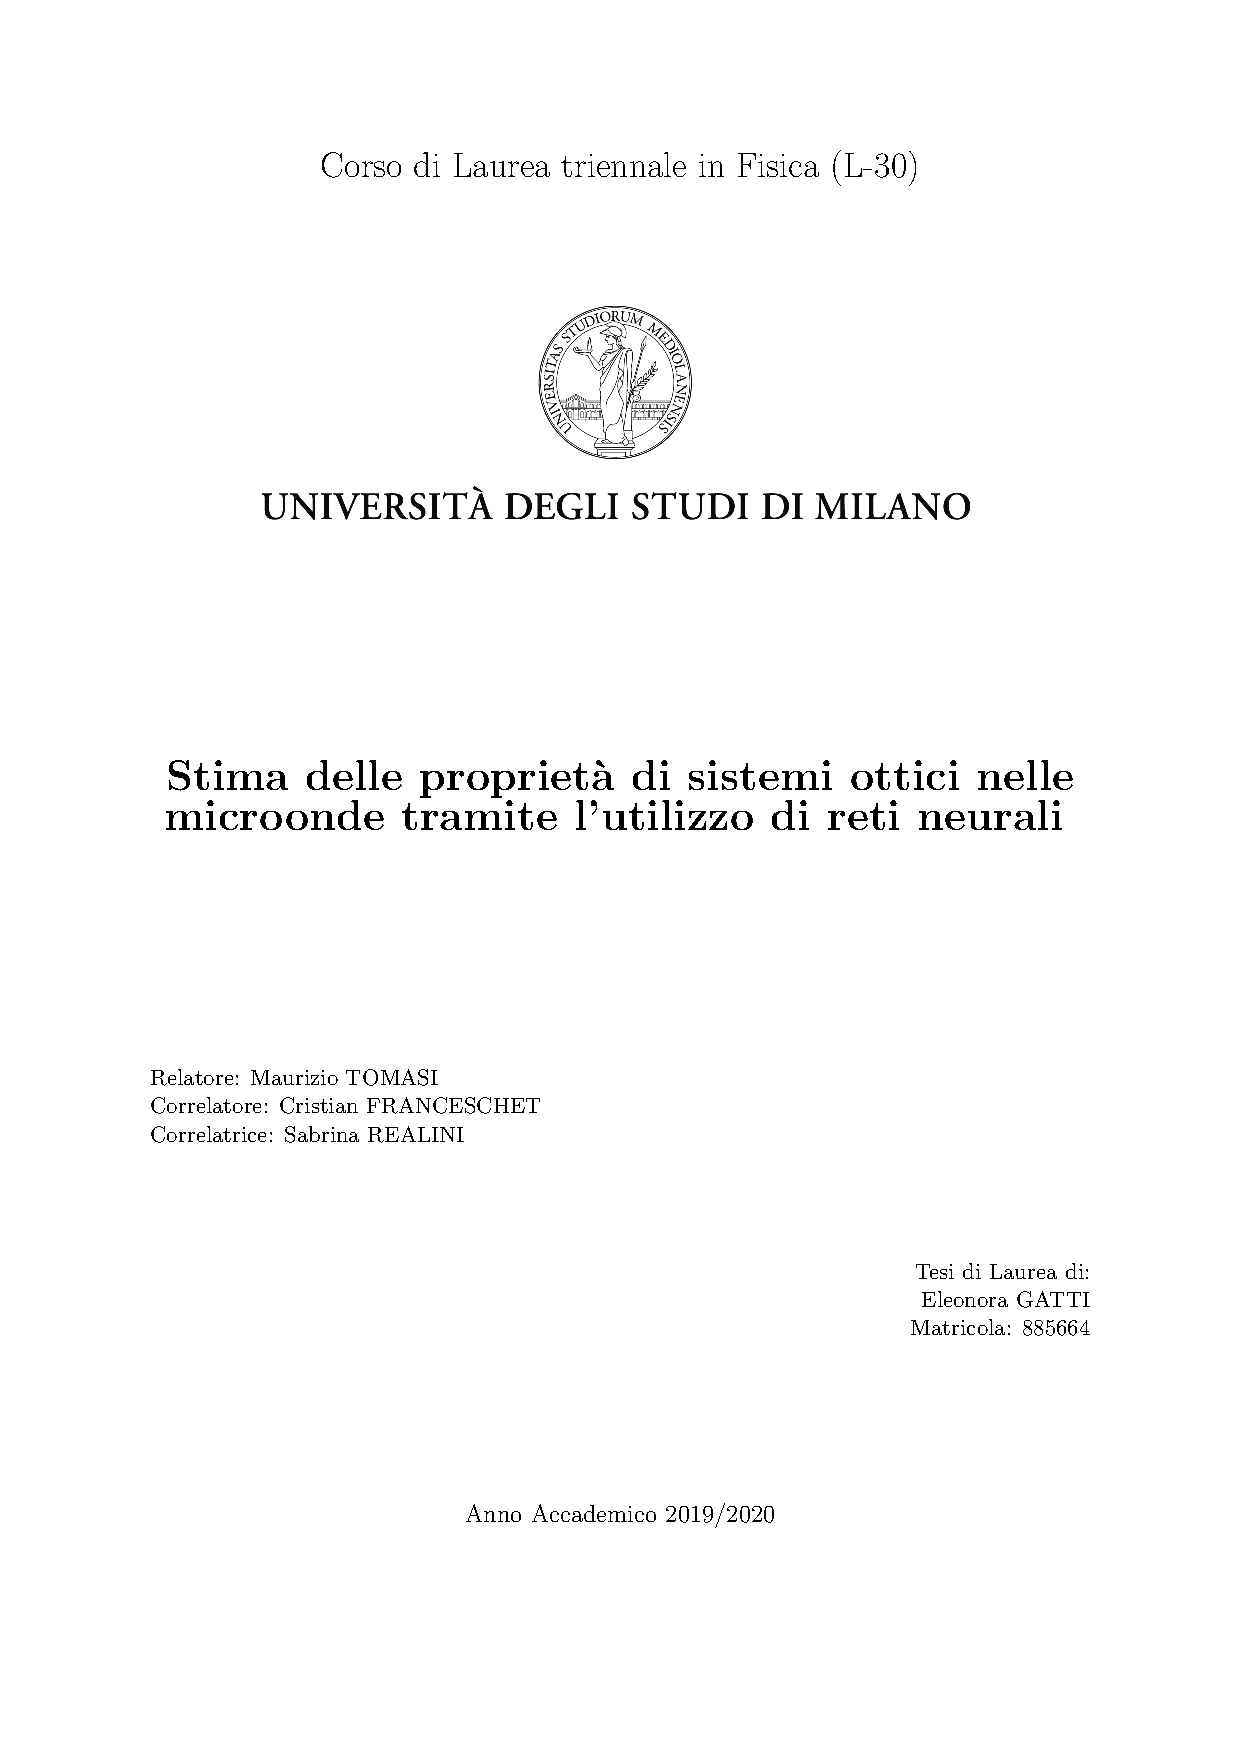
\includepdf[pages=-]{../frontespizio/frontespizio.pdf}
\newpage
\thispagestyle{empty}
\clearpage\mbox{}\clearpage
\newpage
\thispagestyle{empty}

%%%%%%%%%%%%%%%%%%%%%%%  INDICE  %%%%%%%%%%%%%%%%%%%%%

\tableofcontents
\newpage

%%%%%%%%%%%%%%%%%%%%  CAPITOLO 1  %%%%%%%%%%%%%%%%%%%%

\chapter{Sistemi ottici nelle microonde}\label{intro_sistemi_ottici}

    %%%%%%%%%%%%%%%%%%%  CAPITOLO 1.1  %%%%%%%%%%%%%%%%%%%

\section{Utilizzo delle microonde in astrofisica}\label{microonde_astrofisica}

    %%%%%%%%%%%%%%%%%%%  CAPITOLO 1.2  %%%%%%%%%%%%%%%%%%%

\section{Diagramma di radiazione}\label{rad_pattern}

    %%%%%%%%%%%%%%%%%%  CAPITOLO 1.3  %%%%%%%%%%%%%%%%%%%%

\section{Simulazione di sistemi ottici}\label{simulazioni}


%%%%%%%%%%%%%%%%%%%%%%%%%%%%%%%%%%%%%%%%%%%%%%%%%%%%%%%
%%%%%%%%%%%%%%%%%%%%%%%%%%%%%%%%%%%%%%%%%%%%%%%%%%%%%%%
%%%%%%%%%%%%%%%%%%%%%%%%%%%%%%%%%%%%%%%%%%%%%%%%%%%%%%%
%                   FINE CAPITOLO 1                   %
%%%%%%%%%%%%%%%%%%%%%%%%%%%%%%%%%%%%%%%%%%%%%%%%%%%%%%%
%%%%%%%%%%%%%%%%%%%%%%%%%%%%%%%%%%%%%%%%%%%%%%%%%%%%%%%
%%%%%%%%%%%%%%%%%%%%%%%%%%%%%%%%%%%%%%%%%%%%%%%%%%%%%%%


%%%%%%%%%%%%%%%%%%%%  CAPITOLO 2  %%%%%%%%%%%%%%%%%%%%

\chapter{Regressione con reti neurali}\label{reg_nn}
Le reti neurali artificiali rappresentano una tecnica di Machine Learning che si è ampiamente diffusa negli ultimi anni. \\
L'idea utopica su cui si fondano le reti neurali artificiali è quella di simulare il comportamenteo del cervello umano. Questo è un sistema estremamente complesso basato sull'interconnessioni di unità fondamentali: i \textbf {neuroni}. \\

%%%%%%%%%%%%%%%%%%%%%%%%%%%%%%%%%%%%%%%%%%%%%%%%%%%%%%%
%%%%%%%%%%%%%%%%%%%%%%%%%%%%%%%%%%%%%%%%%%%%%%%%%%%%%%%
%%%%%%%%%%%%%%%%%%%%%%%%%%%%%%%%%%%%%%%%%%%%%%%%%%%%%%%
%                   FINE CAPITOLO 2                   %
%%%%%%%%%%%%%%%%%%%%%%%%%%%%%%%%%%%%%%%%%%%%%%%%%%%%%%%
%%%%%%%%%%%%%%%%%%%%%%%%%%%%%%%%%%%%%%%%%%%%%%%%%%%%%%%
%%%%%%%%%%%%%%%%%%%%%%%%%%%%%%%%%%%%%%%%%%%%%%%%%%%%%%%


%%%%%%%%%%%%%%%%%%%%  CAPITOLO 3  %%%%%%%%%%%%%%%%%%%%

\chapter{Previsione delle proprietà di un diagramma di radiazione}\label{prev_param}

    %%%%%%%%%%%%%%%%%%%  CAPITOLO 3.1  %%%%%%%%%%%%%%%%%%%

\section{Interpolazione}\label{interpolazione}

         %%%%%%%%%%%%%%%%%%%  CAPITOLO 3.1.1  %%%%%%%%%%%%%%%%%%%

\subsection{Interp2d}\label{interp2d}

         %%%%%%%%%%%%%%%%%%%  CAPITOLO 3.1.2  %%%%%%%%%%%%%%%%%%%

\subsection{Curve Fit}\label{curve_fit}
        
        %%%%%%%%%%%%%%%%%%%  CAPITOLO 3.1.3  %%%%%%%%%%%%%%%%%%%

\subsection{Risultati dell'interpolazione}\label{risultati_interpolazione}


     %%%%%%%%%%%%%%%%%%%  CAPITOLO 3.2  %%%%%%%%%%%%%%%%%%%
\section{Reti neurali}\label{reti_neurali}

        %%%%%%%%%%%%%%%%%%%  CAPITOLO 3.2.1  %%%%%%%%%%%%%%%%%%%

\subsection{Architettura della rete}\label{architettura}

        %%%%%%%%%%%%%%%%%%%  CAPITOLO 3.2.2  %%%%%%%%%%%%%%%%%%%

\subsection{Pre Training}\label{pre_training}

        %%%%%%%%%%%%%%%%%%%  CAPITOLO 3.2.3  %%%%%%%%%%%%%%%%%%%

\subsection{Training}\label{training}

        %%%%%%%%%%%%%%%%%%%  CAPITOLO 3.2.4  %%%%%%%%%%%%%%%%%%%

\subsection{Risultati delle reti}\label{risultati_reti}

%%%%%%%%%%%%%%%%%%%%%%%%%%%%%%%%%%%%%%%%%%%%%%%%%%%%%%%
%%%%%%%%%%%%%%%%%%%%%%%%%%%%%%%%%%%%%%%%%%%%%%%%%%%%%%%
%%%%%%%%%%%%%%%%%%%%%%%%%%%%%%%%%%%%%%%%%%%%%%%%%%%%%%%
%                   FINE CAPITOLO 3                   %
%%%%%%%%%%%%%%%%%%%%%%%%%%%%%%%%%%%%%%%%%%%%%%%%%%%%%%%
%%%%%%%%%%%%%%%%%%%%%%%%%%%%%%%%%%%%%%%%%%%%%%%%%%%%%%%
%%%%%%%%%%%%%%%%%%%%%%%%%%%%%%%%%%%%%%%%%%%%%%%%%%%%%%%







%%%%%%%%%%%%%%%%%%%%  CAPITOLO 4  %%%%%%%%%%%%%%%%%%%%

\chapter{Conclusioni}\label{conclusioni}

%%%%%%%%%%%%%%%%%%%%%%%%%%%%%%%%%%%%%%%%%%%%%%%%%%%%%%%
%%%%%%%%%%%%%%%%%%%%%%%%%%%%%%%%%%%%%%%%%%%%%%%%%%%%%%%
%%%%%%%%%%%%%%%%%%%%%%%%%%%%%%%%%%%%%%%%%%%%%%%%%%%%%%%
%                   FINE CAPITOLO 4                   %
%%%%%%%%%%%%%%%%%%%%%%%%%%%%%%%%%%%%%%%%%%%%%%%%%%%%%%%
%%%%%%%%%%%%%%%%%%%%%%%%%%%%%%%%%%%%%%%%%%%%%%%%%%%%%%%
%%%%%%%%%%%%%%%%%%%%%%%%%%%%%%%%%%%%%%%%%%%%%%%%%%%%%%%




\end{document}